\documentclass[12pt,a4paper,fleqn]{report}

\usepackage[top=2.5cm,bottom=2.5cm,left=3cm,right=3cm]{geometry}

% دعم العربية (XeLaTeX)
\usepackage{fontspec}

\usepackage{polyglossia}

\usepackage{tikz}
\usepackage{tikz-3dplot}

\usetikzlibrary{arrows.meta}
\usetikzlibrary{3d}


\setmainlanguage[numerals=maghrib]{arabic}
\setotherlanguage{english}

\newfontfamily\arabicfont[Script=Arabic]{Arial}

\newfontfamily\englishfont{Times New Roman}

% تنسيق
\usepackage{setspace}
\onehalfspacing

\usepackage{graphicx}
\usepackage{caption}
\usepackage{booktabs}
\usepackage{hyperref}
\usepackage{titlesec}
\usepackage{imakeidx}
\usepackage{float}
\usepackage{amsmath}


% تحميل ملفاتك
%==================== SETTINGS ====================

% دعم الألوان
\usepackage{xcolor}

% المسافات بين الأسطر
\usepackage{setspace}
\onehalfspacing

% تنسيق الفقرات
\setlength{\parindent}{0pt}
\setlength{\parskip}{6pt}

% دعم الصور
\usepackage{graphicx}
\graphicspath{{images/}}

% الجداول
\usepackage{booktabs}
\usepackage{array}

% تحسين النص
\usepackage{microtype}

% الروابط
\usepackage{hyperref}
\hypersetup{
    colorlinks=true,
    linkcolor=blue,
    filecolor=magenta,
    urlcolor=cyan,
    pdftitle={مشروع التخرج},
    pdfauthor={بهاء الياسين},
    pdfpagemode=FullScreen,
}

% ترقيم الصفحات في الأسفل
\usepackage{fancyhdr}
\pagestyle{fancy}
\fancyhf{}
\fancyfoot[C]{\thepage}

% إزالة الخط العلوي
\renewcommand{\headrulewidth}{0pt}

% دعم القوائم
\usepackage{enumitem}

% دعم الكود البرمجي (اختياري)
\usepackage{listings}

\lstset{
    basicstyle=\ttfamily\small,
    breaklines=true,
    frame=single
}
%==================== STYLES ====================

% تنسيق العناوين
\usepackage{titlesec}

% تنسيق Chapter
\titleformat{\chapter}
{\Huge\bfseries}
{\thechapter}
{1em}
{}

% تنسيق Section
\titleformat{\section}
{\Large\bfseries}
{\thesection}
{1em}
{}

% تنسيق Subsection
\titleformat{\subsection}
{\large\bfseries}
{\thesubsection}
{1em}
{}

% المسافات بين العناوين
\titlespacing*{\chapter}{0pt}{-20pt}{20pt}
\titlespacing*{\section}{0pt}{10pt}{10pt}
\titlespacing*{\subsection}{0pt}{8pt}{8pt}

% تنسيق الفهرس
\usepackage{tocloft}

\renewcommand{\cftchapfont}{\bfseries}
\renewcommand{\cftsecfont}{}
\renewcommand{\cftchappagefont}{\bfseries}

% مسافات الفهرس
\setlength{\cftbeforechapskip}{5pt}

% دعم اتجاه عربي أفضل
%\raggedleft

% تنسيق الصور
\usepackage{caption}
\captionsetup{
    justification=raggedleft,
    singlelinecheck=false
}

% تنسيق الجداول
\renewcommand{\arraystretch}{1.5}

% أوامر مساعدة
\newcommand{\HRule}{\rule{\linewidth}{0.5mm}}

% تحسين عرض الكود
\lstdefinestyle{mystyle}{
    backgroundcolor=\color{gray!10},
    commentstyle=\color{green},
    keywordstyle=\color{blue},
    numberstyle=\tiny\color{gray},
    stringstyle=\color{red},
    basicstyle=\ttfamily\small,
    breaklines=true,
    frame=single
}

\lstset{style=mystyle}

\makeindex[columns=2, title=الفهرس, options= -s resources/styles/indexstyle.ist, intoc]
\indexsetup{level=\chapter*,toclevel=chapter}

%==================== بداية المستند ====================
\begin{document}

%==================== صفحة الغلاف ====================
\makeatletter

\newcommand*{\gradeType}[1]{\gdef\@gradeType{#1}}
\newcommand*{\firstExaminer}[1]{\gdef\@firstExaminer{#1}}
\newcommand*{\secondExaminer}[1]{\gdef\@secondExaminer{#1}}
\newcommand*{\matrikelnr}[1]{\gdef\@matrikelnr{#1}}
\newcommand*{\submitDate}[1]{\gdef\@submitDate{#1}}

\renewcommand*{\maketitle}{
	\begin{titlepage}
		\newgeometry{left=2.5cm,right=2.5cm,top=2.0cm,bottom=2.5cm}
		\begin{center}
			
\includegraphics[width=0.5\textwidth]{resources/images/logo_of_aleppo_uni}				
			\vfill
			{\Large \@title\par}
			\vskip 0.5cm
			{\large \bfseries  أتمتة عملية لمنظومة المقص الطائر \par}
			\vskip 0.5cm
			%{\large مقدم لنيل\\ \bfseries \@gradeType}
			\vskip 0.5cm
			{\large جامعة حلب}
			\vskip 0.5cm
			{\large  كلية الهندسة الكهربائية و الألكترونية\\ قسم هندسة التحكم الآلي والأتمتة الصناعية}
			\vfill
			\begin{flushright}
				\begin{tabular}[t]{rl}
					المشرف: &\@firstExaminer\\
					
					الكاتب: &\@author\\
					الرقم الجامعي : & \@matrikelnr\\
					تاريخ التقديم : & \@submitDate\\
				\end{tabular}
			\end{flushright}
		\end{center}
		\restoregeometry
	\end{titlepage}
}
\makeatother
%\gradeType{درجة البكالوريوس} % مثل: Bachelor of Science, Master of Science, إلخ  
\title{ تقرير عملي}
\firstExaminer{د.أيمن خطاب}
%\secondExaminer{الليث, محمد}
\author{بهاء الياسين}
\matrikelnr{215029}
\submitDate{17.06.2026}


\pagenumbering{alph}
\maketitle


%==================== الفهرس ====================
\tableofcontents
\clearpage

%==================== المحتوى ====================
\pagenumbering{arabic}

\chapter{مقدمة}
\label{ch:flying_shear_intro}

تُعد منظومة "المقص الطائر" (\textenglish{Flying Shear}) من أهم التطبيقات العملية وأكثرها ديناميكية في خطوط الإنتاج المستمرة. تكمن المشكلة الكلاسيكية في هذه الخطوط في ضرورة إيقاف السير الناقل بالكامل في كل مرة يُراد فيها قص المنتج للوصول إلى الطول المطلوب، مما يقلل من كفاءة الإنتاج بشكل حاد ويؤدي إلى هدر زمني وميكانيكي كبير.

يُقدم المقص الطائر حلاً هندسياً جذرياً لهذه المشكلة من خلال الاعتماد على ما يُعرف بمبدأ "التزامن الحركي" (\textenglish{Kinematic Synchronization}). تعتمد هذه الفكرة التكنولوجية على وجود عربة قص تتحرك بشكل موازٍ للمنتج، حيث يتم تسريع العربة حتى تتطابق سرعتها الخطية تماماً مع سرعة السير الناقل. 

عند حدوث هذا التطابق (أي عندما تصبح السرعة النسبية بين الشفرة والمنتج تساوي صفراً)، يتم تفعيل آلية القص والمنتج لا يزال يتحرك بفضل التزامن. بعد إتمام القطع، تُرفع الشفرة وتعود العربة بأقصى سرعة ممكنة إلى نقطة البداية لانتظار القطعة التالية. 

يستعرض هذا التقرير التطبيق العملي لأتمتة هذه المنظومة بشكل متسلسل، حيث تتناول الفصول القادمة تحديد المداخل والمخارج، التوصيل الفيزيائي، الحسابات الديناميكية، وصولاً إلى بناء الخوارزمية البرمجية التي تدير العملية بالكامل.

















\chapter{توزيع المداخل والمخارج}
\label{ch:io_mapping}

لضمان استقرار المنظومة وتجنب أي تعارض في البنية العتادية \textenglish{(Hardware Conflict)} للمتحكم، تمت دراسة وتوزيع المداخل والمخارج بدقة بناءً على المتطلبات الوظيفية للآلة ودليل الشركة المصنعة لمتحكمات دلتا \textenglish{(Delta DVP)}. يعتمد هذا التوزيع على تخصيص قنوات محددة للتعامل مع الإشارات عالية التردد (مثل نبضات المشفر ومخارج السيرفو)، مع ترك المداخل والمخارج العادية لمهام التحكم والحماية الكلاسيكية.

\section{الجدول الشامل للمداخل والمخارج}
يوضح الجدول التالي التوزيع المعتمد في هذه المنظومة لربط الحساسات والمشغلات مع منافذ المتحكم المنطقي:

\begin{table}[h!]
\centering
\renewcommand{\arraystretch}{1.5}
\begin{tabular}{|c|p{11cm}|}
\hline
\textbf{العنوان} & \textbf{الوظيفة الميكانيكية والبرمجية} \\
\hline
\textbf{X0} & مفتاح بدء التشغيل وتفعيل النظام الميكانيكي \textenglish{(System Start)}. \\
\hline
\textbf{X1} & مفتاح الإيقاف العام للمنظومة \textenglish{(System Stop)}. \\
\hline
\textbf{X2} & إشارة الحماية من زيادة الحمل \textenglish{(Overload Protection)} لإيقاف النظام عند حدوث أخطاء كهربائية أو ميكانيكية. \\
\hline
\textbf{X3} & حساس المنتج الضوئي، ويُبرمج كحافة صاعدة \textenglish{(Rising Edge)} لتصفير العداد لمرة واحدة. \\
\hline
\textbf{X4} & قناة الطور الأول للمشفر \textenglish{(Phase A)} - مرتبطة عتادياً بالعداد السريع \textenglish{C254}. \\
\hline
\textbf{X5} & قناة الطور الثاني للمشفر \textenglish{(Phase B)} - مرتبطة عتادياً بالعداد السريع \textenglish{C254}. \\
\hline
\textbf{X6} & حساس نقطة الصفر \textenglish{(Home Sensor)} لإيقاف عربة المقص وتحديد نقطة الانطلاق. \\
\hline
\textbf{X7} & حساس نهاية الشوط الأمامي \textenglish{(Forward Limit Switch)} لعمل كبح طوارئ للمحرك. \\
\hline
\textbf{X10} & حساس نهاية الشوط الخلفي \textenglish{(Reverse Limit Switch)} لعمل كبح طوارئ للمحرك. \\
\hline
\textbf{Y0} & مخرج النبضات عالي التردد \textenglish{(Pulse Output)} للتحكم في سرعة ومسافة السيرفو. \\
\hline
\textbf{Y1} & مخرج تحديد الاتجاه \textenglish{(Direction)} لتمييز التقدم للأمام أو التراجع للخلف. \\
\hline
\textbf{Y2} & إشارة تفعيل محرك السيرفو والمحافظة على المغنطة \textenglish{(Servo Enable / SON)}. \\
\hline
\textbf{Y4} & مخرج تفعيل أسطوانة القص لإنزال السكين في لحظة التزامن. \\
\hline
\end{tabular}
\caption{\centering{توزيع المداخل والمخارج}}
\label{tab:io_mapping}
\end{table}




















\chapter{التوصيل الفيزيائي }
\label{ch:plc_wiring}

لضمان توافق الخوارزمية البرمجية مع الواقع الصناعي، تم تصميم مخطط التوصيل الكهربائي المرجعي لمتحكم \textenglish{DVP-28SV11T} لتُبنى عليه محاكاة النظام، وذلك وفقاً للتوزيع التالي:

\begin{itemize}
    \item \textbf{المشفر القائد:} تُربط قنواته (\LR{A, B}) بالمداخل النبضية السريعة \LR{(X4, X5)} عبر كابلات محمية (\textenglish{Shielded}) لمنع التشويش، ويُوصل الطرف المشترك \LR{(S/S)} بجهد $24\text{ VDC}$.
    \item \textbf{مشغل السيرفو:} يُقاد عبر مخارج الترانزستور وفق بروتوكول (النبضة والاتجاه). يُخصص المخرج \LR{Y0} للنبضات، \LR{Y1} للاتجاه، و \LR{Y2} لإشارة التفعيل (\textenglish{SON}). وتُضاف مقاومة $2.2\text{ k}\Omega$ على التوالي لحماية دوائر السيرفو الداخلية.
    \item \textbf{مفاتيح الحماية:} تُوصل إشارات السلامة ونهايات الشوط \LR{(X1, X2, X7, X10)} كتلامسات مغلقة طبيعياً \LR{(NC)}، مما يضمن التوقف الآمن والمباشر للنظام عند حدوث أي انقطاع في الأسلاك.
\end{itemize}

يوضح الشكل \ref{fig:full_wiring_diagram} أدناه البنية الكهربائية المتكاملة للمنظومة.

\begin{figure}[h!]
    \centering
    \resizebox{\textwidth}{!}{%
    \begin{tikzpicture}[>=stealth, thick, text=black]

    % ==========================================
    % 1. PLC BLOCK
    % ==========================================
    \draw[fill=gray!10, draw=black!80, line width=1.5pt, rounded corners] (5, 0) rectangle (9.5, 13);
    \node[align=center, font=\large\bfseries] at (7.25, 12.2) {Delta PLC \\ \small DVP-28SV11T};
    \draw[line width=1pt, black!50] (5, 11.5) -- (9.5, 11.5);

    % Common 24V Line for Inputs
    \draw[red, line width=1.5pt] (0, 1) -- (0, 11.5) node[above, font=\bfseries] {+24V DC};

    % S/S Terminal
    \node[anchor=west, font=\bfseries] at (5.2, 10.8) {S/S};
    \draw[red, line width=1.2pt, ->] (0, 10.8) -- (5, 10.8);

    % Input Labels Inside PLC
    \foreach \y/\label in {9.5/X0, 8.5/X1, 7.5/X2, 6.5/X3, 5.5/X4, 4.5/X5, 3.5/X6, 2.5/X7, 1.5/X10} {
        \node[anchor=west, font=\bfseries] at (5.2, \y) {\label};
    }

    % ==========================================
    % 2. INPUTS (Drawing Electrical Symbols)
    % ==========================================

    % X0: Start (NO Pushbutton)
    \draw[blue, thick] (0, 9.5) -- (1.5, 9.5);
    \draw[blue, thick, ->] (2.5, 9.5) -- (5, 9.5) node[midway, above, font=\footnotesize] {Start (NO)};
    \filldraw[black] (1.5, 9.5) circle (1.5pt);
    \filldraw[black] (2.5, 9.5) circle (1.5pt);
    \draw[black, thick] (1.5, 9.8) -- (2.5, 9.8); % NO bridge
    \draw[black, thick] (2.0, 9.8) -- (2.0, 10.1); % Plunger

    % X1: Stop (NC Pushbutton)
    \draw[blue, thick] (0, 8.5) -- (1.5, 8.5);
    \draw[blue, thick, ->] (2.5, 8.5) -- (5, 8.5) node[midway, above, font=\footnotesize] {Stop (NC)};
    \filldraw[black] (1.5, 8.5) circle (1.5pt);
    \filldraw[black] (2.5, 8.5) circle (1.5pt);
    \draw[black, thick] (1.5, 8.5) -- (2.5, 8.5); % NC touching
    \draw[black, thick] (2.0, 8.5) -- (2.0, 8.8); % Plunger

    % X2: Thermal Overload (NC)
    \draw[blue, thick] (0, 7.5) -- (1.5, 7.5);
    \draw[blue, thick, ->] (2.5, 7.5) -- (5, 7.5) node[midway, above, font=\footnotesize] {Overload (NC)};
    \filldraw[black] (1.5, 7.5) circle (1.5pt);
    \filldraw[black] (2.5, 7.5) circle (1.5pt);
    \draw[black, thick] (1.5, 7.5) -- (2.5, 7.5); % NC touching
    \draw[black, thick] (1.7, 7.5) -- (1.9, 7.8) -- (2.1, 7.5); % Thermal zigzag symbol
    \draw[black, thick] (2.1, 7.5) -- (2.3, 7.8);

    % X3: Photocell (Sensor Box)
    \draw[blue, thick] (0, 6.5) -- (1.5, 6.5);
    \draw[blue, thick, ->] (2.5, 6.5) -- (5, 6.5) node[midway, above, font=\footnotesize] {Photocell};
    \draw[fill=white, draw=black, thick] (1.5, 6.2) rectangle (2.5, 6.8);
    \node[font=\footnotesize\bfseries] at (2.0, 6.5) {PE};

    % X4, X5: Master Encoder
    \draw[red, thick] (0, 5.0) -- (1.0, 5.0);
    \draw[fill=blue!5, draw=blue!50, thick, rounded corners] (1.0, 4.2) rectangle (2.5, 5.8);
    \node[align=center, font=\footnotesize\bfseries] at (1.75, 5.0) {Master\\Encoder};
    \draw[blue, thick, ->] (2.5, 5.5) -- (5, 5.5) node[midway, above, font=\footnotesize] {Ch A};
    \draw[blue, thick, ->] (2.5, 4.5) -- (5, 4.5) node[midway, above, font=\footnotesize] {Ch B};

    % X6: Home Sensor (Proximity)
    \draw[blue, thick] (0, 3.5) -- (1.5, 3.5);
    \draw[blue, thick, ->] (2.5, 3.5) -- (5, 3.5) node[midway, above, font=\footnotesize] {Home Sens.};
    \draw[fill=white, draw=black, thick] (1.5, 3.2) rectangle (2.5, 3.8);
    \node[font=\footnotesize\bfseries] at (2.0, 3.5) {PRX};

    % X7: Forward Limit (NC Switch)
    \draw[blue, thick] (0, 2.5) -- (1.5, 2.5);
    \draw[blue, thick, ->] (2.5, 2.5) -- (5, 2.5) node[midway, above, font=\footnotesize] {Fwd Limit (NC)};
    \filldraw[black] (1.5, 2.5) circle (1.5pt);
    \filldraw[black] (2.5, 2.5) circle (1.5pt);
    \draw[black, thick] (1.5, 2.5) -- (2.5, 2.5); % NC touching
    \draw[black, thick] (2.0, 2.5) -- (2.0, 2.8);
    \draw[black, thick] (1.8, 2.8) -- (2.2, 2.8); % Roller T-shape

    % X10: Reverse Limit (NC Switch)
    \draw[blue, thick] (0, 1.5) -- (1.5, 1.5);
    \draw[blue, thick, ->] (2.5, 1.5) -- (5, 1.5) node[midway, above, font=\footnotesize] {Rev Limit (NC)};
    \filldraw[black] (1.5, 1.5) circle (1.5pt);
    \filldraw[black] (2.5, 1.5) circle (1.5pt);
    \draw[black, thick] (1.5, 1.5) -- (2.5, 1.5); % NC touching
    \draw[black, thick] (2.0, 1.5) -- (2.0, 1.8);
    \draw[black, thick] (1.8, 1.8) -- (2.2, 1.8); % Roller T-shape

    % ==========================================
    % 3. OUTPUTS
    % ==========================================

    % Output Labels Inside PLC
    \foreach \y/\label in {9.5/Y0 (Pulse), 8.5/Y1 (Dir), 7.5/Y2 (Enable), 4.5/Y4 (Cutter)} {
        \node[anchor=east, font=\bfseries] at (9.3, \y) {\label};
    }

    % Servo Drive Box
    \draw[fill=green!5, draw=green!60!black, rounded corners, thick] (13.5, 7) rectangle (17.5, 10.5);
    \node[align=center, font=\bfseries] at (15.5, 10.0) {Servo Drive};
    
    % Servo Drive Terminals Text
    \node[anchor=west, font=\footnotesize] at (13.6, 9.5) {PULS-};
    \node[anchor=west, font=\footnotesize] at (13.6, 8.5) {SIGN-};
    \node[anchor=west, font=\footnotesize] at (13.6, 7.5) {SON};

    % Servo Wiring with Resistors
    \draw[green!50!black, thick, ->] (9.5, 9.5) -- (13.5, 9.5) node[midway, fill=white, draw=black, inner sep=2pt, font=\footnotesize] {2.2 k$\Omega$};
    \draw[green!50!black, thick, ->] (9.5, 8.5) -- (13.5, 8.5) node[midway, fill=white, draw=black, inner sep=2pt, font=\footnotesize] {2.2 k$\Omega$};
    \draw[green!50!black, thick, ->] (9.5, 7.5) -- (13.5, 7.5);
    
    % Servo +24V Supply
    \draw[red, thick, <-] (14.5, 10.5) -- (14.5, 11.2) node[above, font=\bfseries] {+24V DC};
    
    % Cutter Solenoid Box
    \draw[fill=orange!10, draw=orange!80!black, rounded corners, thick] (13.5, 3.5) rectangle (17.5, 5.5);
    \node[align=center, font=\bfseries] at (15.5, 4.5) {Cutter Solenoid};
    
    % Cutter Wiring
    \draw[orange!80!black, thick, ->] (9.5, 4.5) -- (13.5, 4.5);
    
    % Cutter +24V Supply
    \draw[red, thick, <-] (14.5, 5.5) -- (14.5, 6.2) node[above, font=\bfseries] {+24V DC};

    \end{tikzpicture}
    }
    \caption[المخطط الشامل لتوصيل المداخل والمخارج]{\centering المخطط الشامل لتوصيل المداخل والمخارج مع جهاز الـ \textenglish{PLC} لمنظومة المقص الطائر.}
    \label{fig:full_wiring_diagram}
\end{figure}












\chapter{الحسابات الديناميكية وضبط المعايير}
\label{ch:kinematics}

يُعد هذا الفصل العصب الرياضي لمنظومة المقص الطائر، حيث تُترجم المتطلبات الميكانيكية لسرعة السير وطول المنتج إلى قيم نبضية وترددات يتعامل معها جهاز الـ \textenglish{PLC} لتحقيق التزامن التام.

\section{معايرة المحورين القائد والتابع}
\begin{itemize}
    \item \textbf{المحور القائد (المشفر):} تمت معايرته ليُعطي $1000$ نبضة لكل مسافة $100\text{ mm}$. وبما أن طول المنتج المطلوب هو $200\text{ mm}$، فإن الشرط البرمجي لتفعيل القص هو وصول العداد السريع إلى القيمة التالية:
    $$x = \frac{200\text{ mm} \times 1000\text{ pulses}}{100\text{ mm}} = 2000\text{ pulses}$$

    \item \textbf{المحور التابع (السيرفو):} يحتاج المحرك إلى $10,000$ نبضة لإتمام دورة ميكانيكية تحرك العربة مسافة $10\text{ mm}$. وبالتالي، تكون دقة التموضع:
    $$\text{Pulses per mm} = \frac{10,000\text{ pulses}}{10\text{ mm}} = 1000\text{ pulses/mm}$$
\end{itemize}

\section{تردد المزامنة والتحليل الهندسي}
لتحقيق التزامن، يجب أن تنطلق عربة المقص بسرعة مطابقة تماماً لسرعة السير الناقل والبالغة $150\text{ mm/s}$. يُحسب تردد النبضات اللازم لإرساله من الـ \textenglish{PLC} إلى السيرفو كالتالي:
$$f = 150\text{ mm/s} \times 1000\text{ pulses/mm} = 150,000\text{ Hz}$$

\textbf{خلاصة التحليل:} يعكس هذا التصميم توازناً هندسياً مثالياً؛ فتردد القراءة الداخل للمتحكم من المشفر يبلغ $1500\text{ Hz}$ فقط (سرعة السير $\times$ دقة المشفر)، مما يضمن حصانة عالية ضد التشويش الكهرومغناطيسي (\textenglish{EMI}). في المقابل، يبلغ تردد التحكم الخارج للسيرفو $150\text{ kHz}$ لضمان أقصى درجات النعومة والدقة. كلا الترددين يقعان ضمن الحدود الآمنة للمنافذ العتادية لمتحكم \textenglish{DVP-28SV11T} (أقصاها $200\text{ kHz}$).




















\chapter{بناء الخوارزمية البرمجية}
\label{ch:software_implementation}

تُمثل بيئة \textenglish{WPLSoft} العقل المدبر للمنظومة، حيث تمت كتابة الخوارزمية باستخدام المخطط السلمي \textenglish{(Ladder Diagram)}. تم تصميم الكود ليتعامل مع متغيرات ديناميكية سريعة جداً، مما استدعى استخدام تعليمات متقدمة بحجم 32-بت \textenglish{(Double Word)} لضمان دقة معالجة البيانات وتجنب تجاوز سعة المسجلات \textenglish{(Overflow)} أثناء قراءة المشفر أو إرسال النبضات.

\section{التحليل الهندسي لبنية الكود}
تنقسم الخوارزمية البرمجية إلى أربع كتل وظيفية رئيسية، صُممت كل منها لمعالجة تحدٍ ديناميكي محدد:

\begin{enumerate}
    \item \textbf{العداد السريع والتصفير الذاتي (\textenglish{High-Speed Counter \& Self-Reset}):}
    تم استخدام التعليمة \LR{DCNT C254} لتفعيل قراءة قنوات المشفر القائد باستمرار. ولضمان عدم تراكم الخطأ مع استمرار حركة خط الإنتاج، تم ابتكار حيلة "التصفير الذاتي"، حيث يتم تصفير العداد \LR{C254} باستخدام تعليمة \LR{RST} فوراً في اللحظة الأولى لبدء عملية القطع، لضمان دقة متناهية للقطعة التالية.
    
    \item \textbf{اتخاذ قرار القص (\textenglish{Cutting Decision}):}
    تتم مراقبة القيمة المتراكمة للعداد برمجياً بشكل دائم باستخدام تعليمة المقارنة المزدوجة \LR{DLD>= C254 K2000}. وبمجرد وصول العداد إلى $2000$ نبضة (والتي تكافئ طول الصابون المطلوب $200\text{ mm}$)، تُصدر الخوارزمية إشارة الانطلاق والمزامنة الفورية.
    
    \item \textbf{التزامن الحركي وتوليد النبضات (\textenglish{Pulse Output \& Synchronization}):}
    لتحقيق التطابق الحركي مع السير الناقل، يتم إرسال نبضات عالية التردد لدرايف السيرفو باستخدام التعليمة \LR{DPLSY K150000 K0 Y0}. يضمن هذا التردد ($150\text{ kHz}$) انطلاق المقص وتسارعه حتى يطابق سرعة السير ($150\text{ mm/s}$)، مع الحفاظ على التزامن التام طوال فترة نزول الشفرة.
    
    \item \textbf{شبكات الحماية الميكانيكية (\textenglish{Protection Networks}):}
    تُربط إشارات حساسات نهاية الشوط (\LR{X7, X10}) كشروط أمان قسرية. عند تجاوز العربة لمسارها المسموح، تقوم هذه التماسات بعمل تصفير إجباري (\textenglish{Reset}) لعلامات الحركة (\LR{M1, M2, M3})، مما يقطع النبضات فوراً ويوقف الحركة، مع إبقاء المحرك ممغنطاً لمنع اندفاع العربة بفعل القصور الذاتي.
\end{enumerate}

\begin{figure}[h!]
    \centering
    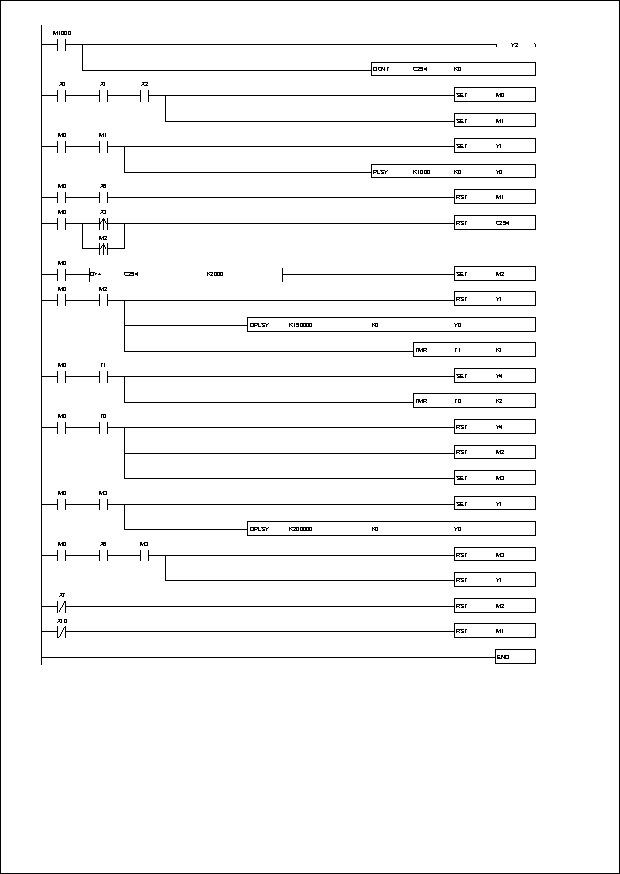
\includegraphics[width=\textwidth]{resources/code/flying_shear_code.pdf} 
    \caption[المخطط السلمي لخوارزمية المقص الطائر]{\centering المخطط السلمي لخوارزمية المقص الطائر في بيئة \textenglish{WPLSoft}، يوضح شبكات المزامنة النبضية والعدادات السريعة وحماية نهايات الشوط.}
    \label{fig:ladder_code}
\end{figure}



\vspace{1cm}
\textbf{لمشاهدة منظومة الآلة عملياً:}
\begin{center}
\LR{https://youtu.be/uw45qdJEOuA}
\end{center}

\end{document}